\secnumbersection{DEFINICIÓN DEL PROBLEMA}

\subsection{DEFINICIÓN}

Actualmente, no existe un procedimiento que permita extraer un set de datos estructurados desde los logs de los UTs.

\subsection{CONTEXTO}

El VLT es uno de los telescopios ópticos más avanzados del mundo, compuesto de 4 UTs, 4 ATs, el VLTI, 1 VISTA y 1 VST\cite{eso2023paranal}.
Perteneciente a la ESO, el observatorio se ubica en el Cerro Paranal en el Norte de Chile, y se dedica principalmente a la búsqueda y estudio de galaxias y otras estructuras interestelares\cite{eso1998vlt}.
Para cumplir con estos objetivos, el VLT debe cumplir con altos estándares tecnológicos, con tal de cumplir la visión de avanzar el entendimiento del Universo mediante la disposición de instalaciones de clase mundial \cite{eso1998vlt}. Dicha responsabilidad recae principalmente en los UTs.

Los UTs son telescopios con una lente principal de 8.2 metros de diámetro cada uno. Cada UT se compone de tres elementos; el M1, el M2 y el M3. Estos componentes estan colocados sobre una montura altazimutal, esto es, una montura que permite la rotación del telescopio en dos ejes perpendiculares: uno vertical y uno horizontal.\cite{eso2011m2}

El M1 es de la lente principal, de forma cóncava, la cual a su vez está compuesta de lentes más pequeñas, distribuidas en forma de dona.
Bajo M1 se encuentran 150 actuadores de fuerza axiales; estos son, propulsores hidráulicos y/o neumáticos, donde cada actuador se encuentra debajo de una lente pequeña respectiva.
Estos actuadores dan a M1 una determinada forma óptica, determinada por el patrón de fuerza presentado por los actuadores\cite{eso1998vlt}.

El M2 consiste de una lente de 0.9 metros de diámetro, montada a una distancia de aproximadamente 12.3 metros de M1 a lo largo del eje azimutal, con la lente de M2 apuntando hacia M1.
M2 está además montado sobre un mecanismo electromecánico que sujeta y controla su inclinación\cite{eso2011m2}. 

El M3 consiste de una lente elíptica de 1.24 metros de diametro mayor con 0.86 metros de diametro menor. Este se ubica dentro de una torre, posicionada en el orificio central del M1.
Este puede rotar alrededor de su eje azimutal\cite{eso2011m1}.

Los UTs pueden trabajar solos o en conjunto; este último modo es llevado a cabo por el VLTI, el cuál recombina la luz obtenida por cuatro telescopios (los cuales pueden ser UTs y/o ATs) de forma simultánea, usando una serie de instrumentos, cada uno encargado de recombinar secciones específicas del espectro electromagnético,
usando la Transformada de Fourier en las imágenes obtenidas. Con este sistema, el diametro total disponible para captar luz es igual a distancia entre los telescopios\cite{eso2023vlti}. 

La forma en la que el UT capta la luz esta reflejada en el Anexo 1. Primero, la luz es captada por M1, el cuál gracias a su forma redirige la luz a M2. Luego M2 vuelve a redirigir la luz a M3, el cuál 
redirige la luz a un punto focal. Desde este punto focal, la luz es procesada por un sensor de frente de onda Shack-Hartmann, y luego estos datos son procesados por un computador central\cite{eso1998vlt}.

Al final de este procedimiento, el computador puede detectar aberraciones en la imagen. Esto se detecta usando la imagen de una estrella, desde ahora denominada Estrella Guía, y analizando el offset de dicha Estrella en la imagen usando una prueba polinomial quasi-Zernike.
A partir de dicho offset, el sistema cambia la forma óptica de M1, redistribuyendo el patrón de fuerza a lo largo de los acutadores axiales bajo M1\cite{wilson1987active}.

Una vez terminado este reajuste, se vuelve a captar una imagen de la Estrella Guía y se repite este procedimiento hasta alcanzar una imagen con calidad óptima.

El procedimiento descrito anteriormente se denomina Óptica Activa\cite{eso1998vlt}.

La Óptica Activa permite mitigar las aberraciones y degradación en la calidad de imagen causada por factores como distorsiones térmicas, turbulencia atmosférica, deformación de espejo por ráfagas de viento, errores de manufactura y mantenimiento del telescopio, entre otros.
La Óptica Activa está presente en los M1 de todos los UTs, sin embargo otros instrumentos también pueden disponer de este sistema. Para el caso de esta memoria, se tomará en cuenta
solo la Óptica Activa para M1, los cuales principalmente se encargan de compensar las aberraciones de baja frecuencia\cite{wilson1987active}.

\subsection{ACTORES INVOLUCRADOS}

Los actores involucrados en el problema corresponden a los elementos participantes en el sistema de Óptima Activa del telescopio VLT, más especificamente la célula M1, los sensores de frente de onda Shack-Hartmann y el software de control que almacena y analiza los logs y los datos entregados por los sensores\cite{eso2011vlt}.

\subsection{DIFICULTADES}

Actualmente, los datos retornados por el sistema de Óptica Activa usan un formato abstracto y poco estructurado. Esto también aplica para los logs retornados durante las operaciones dentro del sistema.
Esta falta de estructura imposibilita el análisis de datos, ya que el costo para reordenar y organizar los datos acorde a lo necesitado supera los beneficios del análisis mismo. 

\subsection{OBJETIVOS Y ALCANCE}

EL objetivo detrás de la solución busca desarrollar un procedimiento para extraer los datos no estructurados, transformarlos en datos estructurados, y disponerlos para distintos modelos y sistemas
que buquen analizar dichos datos con diversos fines, como por ejemplo mantenimiento o técnicas de softcomputing.

\subsection{ARBOL DE PROBLEMA}

\vspace{0.5cm}
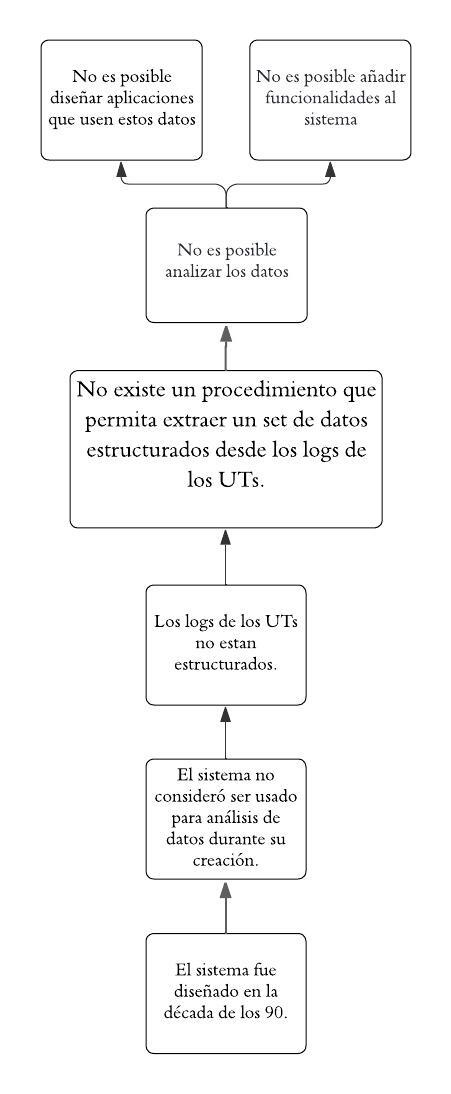
\includegraphics[width=9.5cm,height=16cm]{figures/arbol_problema.jpeg} \\
\vspace{3.5cm}